\documentclass[12pt]{article}
 \usepackage[german]{babel}
 \usepackage[utf8]{inputenc}
 \usepackage{listings}
  \usepackage{color}
  \usepackage{hyperref}
 \usepackage{graphicx}
 \author{Denis Herdt, Almin Causevic}
 \title{ROS auf dem Rapberry Pi}
 \setlength{\parindent}{0pt}
 \setlength{\parskip}{5pt plus 2pt minus 1pt}
 \frenchspacing
 \sloppy
  \lstset{
   basicstyle=\small\ttfamily,
   keywordstyle=\bfseries\ttfamily\color{orange},
   stringstyle=\color{green}\ttfamily,
   commentstyle=\color{middlegray}\ttfamily,
   emph={square}, 
   emphstyle=\color{blue}\texttt,
   emph={[2]root,base},
   emphstyle={[2]\color{black}\texttt},
   showstringspaces=false,
   flexiblecolumns=false,
   tabsize=2,
   frame=tblr
   numbers=left,
   numberstyle=\tiny,
   numberblanklines=false,
   stepnumber=1,
   numbersep=10pt,
   xleftmargin=15pt
 }
 
 
\begin{document}

\begin{figure}[h]


\includegraphics[width=4cm]{hs-logo.jpg}
\end{figure}
Fakultät für Elektrotechnik und Informatik

\vspace{3cm}

\begin{center}

{\bf \huge ROS auf dem Raspberry Pi}
\vspace{4cm}

14 November, 2013
\vspace{1cm}

Systemadministration Projekt in Angewandter Informatik \\
von Denis Herdt und Almin Causevic

\end{center}

\pagebreak

\tableofcontents

\pagebreak

\section{Einleitung}

\subsection{Motivation}

Die Entscheidung für dieses Thema fiel dadurch, dass es zukünftig genutzt werden kann und die Arbeit mit Soft-/Hardware kombiniert wird.

Im Robotiklabor der Hochschule Weingarten wird außerdem zur Zeit noch umständlich ein zusätzlicher Laptop zur Steuerung der Roboter verwendet. Ein Beispiel dafür ist der ''Volksbot''. Durch den Raspberry Pi ergeben sich etliche Vorteile.

Mithilfe des Software-Frameworks ROS (Robot Operating System) kann ein flexibles Netzwerk von Komponenten realisiert werden, in welches der Raspberry eingebunden wird. Dies ist eine einfache und schnelle Methode, eine Robotersteuerung realisieren zu können. ROS wird weltweit eingesetzt und kann auch in Zukunft sehr nützlich sein.

Durch die Kombination mit der Mächtigkeit und Flexibilität von ROS und der gerinen Größe und niedrigen Energieverbrauch des Pi eröffnen sich neue und effiziente Einsatzmöglichkeiten.

Zudem ist dieses Projekt für das Fach Systemadministration sinnvoll, weil mit Linux gearbeitet wird und viel Konfiguration des Betriebssystems vorausgesetzt wird.

\subsection{Zielsetzung}


Unser Hauptziel besteht darin, ROS auf dem Raspberry Pi aufzusetzen und zu nutzen. Dieses Ziel wird wie folgt unterteilt:\\

\begin{itemize}

\item Recherche über Linux Systeme auf dem Raspberry Pi 
\item Passendes Linux System auf Raspberry Pi aufsetzten			
\item Recherche über ROS
\item Geeigneten Roboter wählen (Recherche Verfügbarkeit, Komponenten etc.)
\item Komponenten geschaffen (Wlan Stick, Akkupack, etc.)
\item ROS auf Raspberry Pi aufsetzen
\item Netzwerk zwischen mehreren ROS-Komponenten herstellen
\item Netzwerk mithilfe von Testausgaben überprüfen

\end{itemize}

Mit diesen Zielen ist eine Grundlage für weitere Anwendungen mit ROS auf dem Raspberry geschaffen.\\

{\bf optional}

Da uns am Ende noch genügend Zeit zur Verfügung stand, haben wir folgende Punkte bearbeitet:

\begin{itemize}

\item Steuerungspaket für ''Volksbot'' einbinden
\item Verbesserung der Usability durch Smartphone-Steuerung
\item Optimierung der WLAN-Verbindung am Raspberry
 
\end{itemize}
Bleibt am Ende noch genug Zeit, wird die integriete Kamera des Roboters angesprochen und das Bild mithilfe des Netzwerkes auf einen externen Bildschirm übertragen.
ers soll durch das Schwenken des Smartphones bestimmt werden.

\subsection{Eigene Leistung}

Das ''neue'' an diesem Projekt bezieht sich
auf die Ablösung eines Laptops durch den kleineren und leichteren Raspberry Pi als ROS-Komponente am ausgewählten Roboter. Desweiteren möchten wir herausfinden, ob die Leistung des Pi für diese Aufgabe ausreicht.

\subsection{Aufbau der Arbeit}

In den Grundlagen werden alle wichtigen Komponenten und Aspekte genauer erklärt. Anschließend wird das Grundproblem, welches wir lösen wollen, erläutert und verwandte Arbeiten aufgelistet. 
Darauf folgend werden die dadurch entstandenen Anforderungen und Lösungsvorschläge, sowie die Implementation beschrieben.

\section{Grundlagen}


\subsection{Raspberry Pi Hardwarekomponenten}

"Der Raspberry Pi ist ein kreditkartengroßer Einplatinencomputer, der von der Raspberry Pi Foundation entwickelt wurde" \cite{Pi}
Wir benutzen für dieses Projekt das leistungsstärkere Modell B.
\parbox{7,8cm}{
Technische Details: \cite{Amazon}
\begin{itemize}
\item Preis: ca. 35 Euro
\item Prozessor: ARM1176JZF-S(700 MHz)
\item Broadcom VideoCore IV
\item SDRAM: 512 MB
\item Bis zu 16 GPIO-Pins
\item USB-Anschlüsse: 2
\item FBAS, HDMI
\end{itemize}
}
\parbox{5cm}{
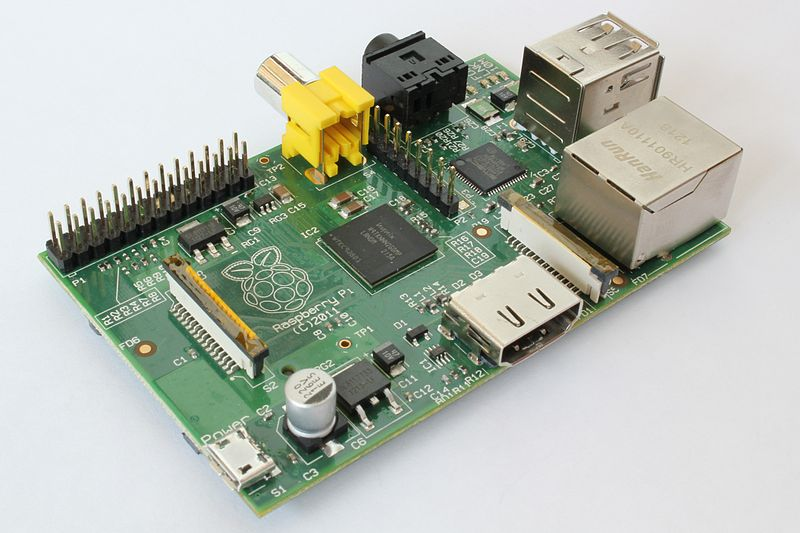
\includegraphics[width=8cm]{Raspi.jpg} \cite{Pipic}
}
\begin{itemize}
\item 3,5-mm-Klinkenstecker (analog), HDMI (digital)
\item Kartenleser für SD (SDHC und SDXC)/MMC/SDIO
\item 10/100-MBit-Ethernet-Controller 
\item 5 V, 700 mA (3,5 Watt)
\item 5-V-Micro-USB-Anschluss (Micro-B), alternativ 4 x AA-Batterien
\end{itemize}

{\bf Stromquelle} Als Stromquelle steht ein Akkupack zum Einsatz. \\
Hierbei ist wichtig, dass der Raspberry mind. 700 mA, besser 1 A zur Stromversorgung bekommt. 
Bei niedrigerer Amperzahl arbeitet der PC oft nicht zuverlässig.

{\bf RAM} Das Model B bietet einen schnelleren und größeren RAM Speicher. Dieser ist wichtig, da viele Signale, teils sogar synchron, verarbeitet werden müssen.

{\bf Datenübertragung} Für die Datenübertragung über das Netz wird ein Standard 300Mbit/s Wlan-Stick benutzt.

{\bf Prozessor} Der Raspberry Pi arbeitet mit einer ARM-Prozessorarchitektur.
Diese Architektur wird gerne für embedded Systems, wie PDAs oder Router, eingesetzt. Diese ist auch auf jedem Smartphone zu finden, da sie den Vorteil einer sehr geringen Leistungsaufnahme bietet. \cite{ARM}

{\bf Betriebssystem} Das auf Linux basierende Betriebssystem Raspbian wird verwendet.
Dabei handelt es sich um ein für Raspberry Pi optimiertes Open-source Debian-System.
Es enthält viele für die ARM-Architektur vorkompilierte Pakete (über 35.000), dazu auch weitere Features, wie etwa eine GUI. \cite{Raspbian}

{\bf GPIO} GPIO (General Purpose Input/Output) ist ein weiteres interessantes Feature des Raspberry Pi.
Es gibt die Möglichkeit, jegliche Hardware-Funktionalität anzusteuern.
Beispielsweise können LED-Leuchten oder der Start-Knopf einer Kaffeemaschine damit über ROS gesteuert werden.
Dies bietet Anreiz für noch mehr Ansätze und Umsetzungen mithilfe des Raspberry Pi und ROS.

\subsection{ROS} 
ROS ist kein eigentliches Betriebssystem im herkömmlichem Sinne, sondern eine Art strukturierte Kommunikationsschicht.
Die Ziele von ROS können zusammengefasst werden zu:
\begin{itemize}
\item Peer-to-peer (System mit vielen laufenden Prozessen auf verschiedenen Hosts)
\item Tool-based (Microkernel-Design bestehend aus vielen Komponenten)
\item multi-lingual (unterstützt viele Computersprachen, z. B. Python, C++, etc.)
\item thin (Wiederverwendbarkeit von Code steht im Mittelpunkt)
\item open source and free (unter der BSD Lizenz) \cite{SLAM}
\end{itemize}
Es ist das einzig existierende Framework, welches sich auf diese Kriterien spezialisiert.
Den Entwicklern von ROS ging es vor allem um die Vereinfachung, Software für eine hohe Zahl an unterschiedlichen Robotern zu schreiben. \\
ROS stellt dazu Bibliotheken, Werkzeuge, Hardware Abstraktion, Gerätetreiber, Bibliotheken, Visualisierungen, Nachrichtenvermittlung, Packetverwaltung und andere Komponenten zur Verfügung. \cite{ROSdescr}
Im Nachfolgenden werden die für dieses Projekt wichtigsten ROS Komponenten kurz beschrieben.

{\bf Topic} Topics können als ''named bus'' gesehen werden, über welche Nodes Messages verteilen können. Es ähnelt dem Multicasting Prinzip. An Topics kann subscribed (zugehört) oder published (geredet) werden.

{\bf Node} Eine Node ist ein simples Programm, welches jede Funktionalität ermöglicht.  Sie kommunizieren direkt über Topics.

{\bf Roscore} Der Roscore kann als Rückgrat des ROS Systems beschrieben werden. Es verwaltet die Registrierung der Nodes und Funktionen in einer Art lookup service für andere Nodes. Es bietet zusätzlich einen Parameter Server, in welchem im laufenden Betrieb Variablen und Paramater gespeichert werden können.

{\bf Package} Software in ROS wird mithilfe von Packages verwaltet.
Sie enthalten Nodes, datasets, configuration files, etc.

{\bf Launchfile} Ein Launchfile ist eine simple XML Datei, welche Informationen über die zu Beginn zu startenden Nodes mit entsprechenden Parametern enthält.
Dies bietet eine komfortablere Alternative, als jedes Node einzeln zu starten.
Ein Beispiel für ein Launchfile ist in der Implementation bei der Steuerung eines Roboters (Volksbot) gegeben. \cite{SLAM}
 
{\bf catkin} Catkin wird in ROS seit der Distribution Groovy als Workspace-Verwaltungssystem verwendet.
Es ist in 4 Spaces unterteilt:
\begin{itemize}
\item Source Space
\item Build Space
\item Devel Space
\item Install Space
\end{itemize}
Catkin bietet uns eine komfortable Möglichkeit über cmake ROS Packages zu compilieren, Tests an ihnen durchzuführen und sie schließlich zu installieren.

\subsection{Volksbot}
\parbox{8cm}{
"VolksBot ist ein Roboterbaukastensystem[...]
Mit Hilfe des Baukastens können sehr schnell und preiswert unterschiedlichste Varianten mobiler Roboter hergestellt werden." \cite{Volksbot}
Der Volksbot wurde an der Hochschule Weingarten für den RoboCup verwendet.
}\hfill
\parbox{5cm}{
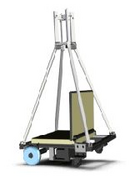
\includegraphics[width=5cm]{Volksbot.jpg} \cite{Volksbotpic}
}
\subsection{Smartphone}

Es wird ein auf Android basierendes Smartphone verwendet.
Wir benutzen auf dem Smartphone eine in einer Projekt-Arbeit entstandene App. \cite{TeleopApp}
Sie bindet sich an einen ROS-Master (später näher erläutert) und übergibt die X- und Y Koordinaten relativ zu sich weiter.
Diese Werte können für die Steuerung des Motors verwendet werden, indem jeweils ein Wert an eine Radachse geliefert wird. Dieser Wert bildet die Geschwindigkeit des Rades ab.
Zur erleichterten Bedienung stellt uns die App eine GUI zur Verfügung. 

\section{Problem}

Viele der heutigen Roboter mit ROS-Systemen besitzen einen leistungsstarken und klobigen PC an Ihrer Seite.
Doch für viele Roboteranwendungen würde auch ein kleinerer, leistungschwächerer PC ausreichen.
Dadurch ergeben sich neue Vorteile:

\begin{itemize}
\item weniger Gewicht
\item weniger Kosten
\item Energieverbrauch sinkt $\rightarrow$ Akku hält länger
\item Die Größe des Roboters nimmt ab
\end{itemize}

Der Roboter Volksbot wird mit einem für diesen Zweck überdimensionierten Laptop gesteuert. Diese Probleme sollen behoben und die obigen Vorteile verschafft werden, indem ROS auf einem Raspberry Pi aufgesetzt wird.

\section{Verwandte Arbeiten}

Master-Thesis:
\begin{enumerate}

\item Robot Navigation in Unknown Environment Based on Combined 2D and 3D Information, Marc Götz, August 2013
\item Semi-Autonomous Grasping of Unknown Objects, Steffen Pfiffner, November 2013
\end{enumerate}

\section{Anforderungen}

Dieses Projekt hat das Ziel, dass ROS auf dem Pi getestet und an einem gegebenen Roboter angewendet wird. Aus diesem Ziel, sowie den vorangegangenen Punkten, erschließen sich folgende Anforderungen:
\vspace{0,4cm}
\begin{itemize}
\item Datenpakete über das ROS-Netzwerk verschicken
\item Robuste und zuverlässige Kommunikation
\item Modulares und flexibles Netzwerk
\item packages sollen leicht in Projekte eingebunden werden

\end{itemize}

{\bf optional}
\begin{itemize}

\item Roboter soll bei Steuerung in die richtige Richtungen fahren
\item Roboter soll sofort auf Anweisungen reagieren
\item Sensibilität der Steuerung sollte einstellbar sein
\item Steuerung über WLAN
\item ROS-Core des Raspberry beim Hochfahren automatisch starten
\item Leichte Bedienbarkeit des Roboters
\item Streaming-Bild ruckelfrei verarbeiten
\item unkonvertiert Echtzeitübertragung
\item Ausgabe am externem Bildschirm
\end{itemize}


\section{Lösungsvorschläge}

{\bf Datenpakete über das Netzwerk verschicken:}\\
Es wird ein ROS-Master aufgesetzt. Dieser gilt als Knotenpunkt (vergleichbar mit einem Defaultgateway) und sorgt für die Kommunikationsmöglichkeit im ROS-Netzwerk.

{\bf Zuverlässige Kommunikation:}\\
Die Netzwerkstabilität und -zuverlässigkeit könnte durch Begrenzung der zeitgleichen Datenübertragung umgesetzt werden. Zusätzlich kann man eine vorangehende Überprüfung der verschickten und erwarteten Datentypen einbinden.

{\bf Flexibles Netzwerk, Packageeinbindung:}\\
Ein modulares und flexibles Netzwerk, sowie das einfache Einbinden von packages ist durch ROS in Kombination mit Catkin gegeben.

{\bf optional}

{\bf Steuerung eines Roboters:}\\
Die Reaktionszeit und Steuerung wird durch zuverlässige und leistungstarke Hardware, sowie durch einen effizient geschriebenen Code bestimmt. In diesem Fall kann die Hardware (mit Ausnahme des Pi) aufrüsten. Der Code lässt sich gar nicht oder nur mühsam verändern und austauschen.

{\bf ROS-Core automatisch starten:}\\
Um bequem mit dem Raspberry arbeiten zu können, ohne jedes mal den ROS-Core starten zu müssen, muss dieser in den Bootvorgang des Raspbian eingebunden werden.

{\bf Leichte Bedienbarkeit:}\\
Diesen Punkt wird mit einer Smartphone App realisieren. Der Roboter soll dabei auf das Schwenken des Smartphones reagieren und seine Geschwindigkeit/Richtung entsprechend anpassen.

{\bf Videoübertragung:}\\
Ein sauberes und störungsfreies Übertragungsbild hängt hauptsächlich von der Hardware des Raspberry Pi, aber auch von der Codierung ab. Der Stream soll durch  Umleiten des Bildes über das Netzwerk an einen PC-Monitor realisiert werden. Falls dabei Probleme auftreten sollten, kann versucht werden, die Codierung zu bearbeiten oder leistungsverstärkende Hardware an den Pi anzuschließen.

\section{Bewertung der Lösungen}

Bis jetzt sind die Lösungsansätze relativ erfolgreich gewesen. Abgesehen von kleineren Leistungsproblemen durch Datenübertragung über das Wlan-Netzwerk, konnten alle Anforderungen gut erfüllt werden.

\section{Implementation}

\subsection{Raspbian}

Zuerst wird das Betriebssystem Raspbian auf dem Pi aufgesetzt.
Hierzu gibt es 2 mögliche Vorgehensweisen:
\begin{enumerate}
\item Installation mit NOOBS
\item Flashen der SD-Karte (Linux mittels dd)
\end{enumerate}

Es wurde die 2. Methode gewählt, da NOOBS 6 verschiedene Images anbietet, doch in diesem Fall nur Raspbian benötigt wird.
Zudem erfordert die 2. Vorgehensweise mehr Arbeit mit dem Linux Betriebssystem, was in dieser Vorlesung nur vorteilhaft sein kann.
Die genauen Installationsschritte werden dem Unterpunkt ''Using the Linux command line'' entnommen. \cite{SDCard}
\\
Um mögliche Fehlerquellen schon beim Herunterladen der Image Datei zu vermeiden, wird empfohlen, wie in der Anleitung beschrieben, die sha1sum zu vergleichen.
%\begin{enumerate}
%\item Mit df -h herausfinden, welchen Namen die SD-Karte trägt (z. B. sdb)
%\item mit dd bs=4M if=~/2012-12-16-wheezy-raspbian.img of=/dev/sdd Image %auf SD-Karte schreiben
%\end{enumerate}

Nun muss nur noch die SD-Karte in den Raspberry eingesteckt werden. Falls eine grüne Leuchte am Raspberry blinkt oder eine Bildschirmausgabe an einem Monitor erscheint, ist dieser Schritt gelungen.

\subsection{ROS aufsetzen}
Der Hersteller Willow Garage stellt seit der Entstehung von ROS mehrerere Distributionen zur Verfügung.
Für den Raspian ist die momentan zweitaktuellste Distribution Groovy zu empfehlen. 
Die aktuelle Version Hydro wird noch nicht unterstützt. \\
Es gibt 2 sinnvolle Wege, ROS Groovy auf dem Raspbian System aufzusetzen.
%Vorteile, Nachteile
\begin{enumerate}
\item Source packages des ROS-Kerns kompilieren
\item binary packages für die ARM-Architektur installieren
\end{enumerate}

Da die Installation und das Kompilieren von Source zwar lehrreich, doch auch relativ zeitaufwendig ist, werden die vorhandenen binary packages für ARM benutzt.
Hierfür nach Punkt 2 der Anleitung vorgehen \cite{RosInstall} \\
Leider werden dadurch nur die grundlegendsten Packages von ROS unterstützt.
Da ein großer Vorteil von ROS die Modularität ist, können leicht benötigte packages über catkin nachinstalliert werden.
Dazu wird später die Vorgehensweise am Beispiel des packages zur Steuerung des Roboters erklärt.\\
\\
%welche, näher erläutern, sourcen
ROS integriert sich sehr gut in die Shell des Linux Systems.
Unterstützt werden mehrere Shell-Typen. In diesem Projekt wird die Bourne Again Shell verwendet.
ROS bietet für seine Systemumgebung Äquivalente zu den wichtigsten Shell Befehlen, beispielsweise roscd für cd oder rosls für ls. \\
Dadurch ergibt sich der Vorteil, nicht den vollständigen Pfad zu einem ROS package oder Verzeichnis eingeben zu müssen. Beispielsweise ist es möglich sofort in ein ROS Verzeichnis mit roscd zu wechseln, ohne den vollständigen Pfad mittels cd eingeben zu müssen. \\
Damit man auf die ROS-typischen Shell Befehle Zugriff hat, muss zuerst gesourced werden.

 \begin{lstlisting}
 source /opt/ros/groovy/setup.bash
 \end{lstlisting}

Der Source Befehl bewirkt, dass die Pfade zu den ROS Verzeichnissen dem Linux System bekannt gemacht werden.
%TODO hier vllt. Bild des Inhaltes von ROS
%Shell Bilder, Bsp. von Kommandos
%TODO in .bashrc eintragen!!

Es empfiehlt sich, sich mit den typischen ROS Befehlen etwas vertraut zu machen. 
Siehe dazu \cite{RosTuts}. \\
Mit diesen Einstellungen sollte es kein Problem mehr sein, ein Netzwerk zwischen Systemen aufzusetzen.
\subsection{Netzwerk aufsetzen}
%Vorrausetzungen für das ROS Netzwerk
Damit ein Netzwerk aufgesetzt werden kann, muss ein Linuxsystem zum Master werden.
%Zu diesem Zweck gehen Sie bitte nach diesem Tutorial vor (Quelle %http://wiki.ros.org/ROS/Tutorials/MultipleMachines)
Im Grunde ist es wichtig, in allen Systemen des Netzwerks in export die IP-Adresse und die Port-Nummer (Standard: 11311) des Systems anzugeben, welches als Master dienen soll.
Hierzu kann man mithilfe des Befehls 

 \begin{lstlisting}
 export ROS_MASTER_URI="http://IP-ADRESSE:11311"
 \end{lstlisting}

die IP-Adresse des Masters angeben.

Eine der Möglichkeiten sich die IP-Adresse des Systems anzeigen zu lassen ist der Shell Befehl ifconfig.

{\bf ROS Workspace anlegen:}

Für ROS sollte noch ein Workspace mit catkin erzeugt werden.
Anleitung dazu unter Punkt 4 der Quelle \cite{Workspace}.
Auch das Sourcen des Workspace sollte am Besten in die .bashrc, aufgenommen werden. \\
Es soll noch zusätzlich ein Beispiel package erzeugt, welches später zum Testen des Netzwerks erforderlich ist.
Dazu in das Source Verzeichnis des catkin Workspace wechseln

 \begin{lstlisting}
 cd ~/catkin_ws/src
 \end{lstlisting}

und ein package erzeugen. 

 \begin{lstlisting}
 catkin_create_pkg beginner_tutorials
 std_msgs rospy roscpp
 \end{lstlisting}

Das package sollte noch compiliert werden.
Erneut in  das catkin Workspace wechseln

 \begin{lstlisting}
 cd ~/catkin_ws
 \end{lstlisting}

und  
 
 \begin{lstlisting}
 catkin_make
 \end{lstlisting}
 
ausführen.
%Für uns ist der Befehl roscore wichtig.
%Wir setzen in unserer exports Datei die ROS!MASTER!URI IP-Adresse auf die %des Raspberry Pi und dazu den Standardport 11311.
%Dies macht den Raspberry zum Master Knotenpunkt, nun können andere Linux-%Systeme mit ROS über diesen kommunizieren.
%Sie müssen zusätzlich in der exports die ROS!MASTER!URI IP-Adresse des %Raspberry angeben.
\subsection{Testen des Netzwerks}

Um das bestehende Netzwerk zu testen, können Datenpakete zwischen den Systemen verschickt werden.
Zuerst sollte der Master ansprechbar sein.
Hierfür wird der Kern von ROS mit dem Shell Befehl 

 \begin{lstlisting}
 roscore
 \end{lstlisting}

gestartet. \\
%TODO Bild der Ausgabe des Kerns mit Highlighting der IP URI
Falls bei Eingabe des Befehls

 \begin{lstlisting}
 rosnode list
 \end{lstlisting}

als Antwort mindestens ein Node (/rosout) erscheint, läuft der Kern ordnungsgemäß. \\
Um nun einfache Testausgaben zwischen Systemen zu schicken, werden zwei ROS Nodes und ein Topic zur Kommunikation eingerichtet.
Auf dem ROS Master wird ein listener Node (Subscriber) gestartet.
Auf einem anderen ROS System wird ein talker Node (Publisher) gestartet. \\ Der Quellcode kann hier heruntergeladen werden \cite{PythonCode}.  \\
Es kann auch der talker anstatt des listeners auf dem Master ausgeführt werden. \\
Es sollte nicht vergessen werden, die Quelldateien mittels

 \begin{lstlisting}
 chmod +x Dateiname.py
 \end{lstlisting}

ausführbar zu machen. \\
{\bf Alternative:} C++ Code \cite{C++Code} \\
\\
Die Nodes mit dem Befehl 

 \begin{lstlisting}
 rosrun beginner_tutorials Dateiname.py
 \end{lstlisting}
 
starten.
Im Shell Fenster des Listener Nodes sollte nun die Ausgabe des Talker Nodes erscheinen.

%Bild einfügen
Falls dies nicht passiert, sollte die obige Anleitung noch einmal genau befolgt werden und zusätzlich das Netzwerk auf Fehler überprüft werden.
\cite{NetworkSetup}

%TODO Auf dem Raspberry nicht möglich?=???!!!
Die Nodes und Topics können zum besseren Verständnis visualisiert werden.
Zuerst muss das rqt package installiert werden.

 \begin{lstlisting}
 sudo get-apt install ros-groovy-rqt
 \end{lstlisting}

Mit 

 \begin{lstlisting}
 rqt_graph 
 \end{lstlisting}

wird das Verhältnis der Nodes visualisiert.

%TODO evtl bild einfügen?

%Hierzu schicken wir mithilfe der App eine Message, welche die X und Y %Koordinaten enthält.

%Wir geben in der App die IP des Masters (Pi) an. Das Handy fungiert nun %als ROS Node und versendet (publish) diese Messages über einen Topic, an %welchem der Pi horcht (subscribe).

%Raspberry Pi kann nun mithilfe des ROS Befehls

%	rostopic echo ''Topicbezeichnung''
	
%aus diesem Topic alle Daten auslesen und ausgeben.
%Bilder der Testdaten
%Da die Koordinaten mit denen auf dem Handy übereinstimmen, ist der %Netzwerktest erfoglreich.

%kurze Info zu Services und Massages, hier wird nicht näher darauf eingegangen!!
%Link zu einem Tutorial bei Interesse
\subsection{Steuerung des Volksbot}

Da der Roboter frei mit dem Smartphone gesteuert werden soll und sich der Raspberry losgelöst auf dem Volksbot befinden soll, werden hierfür Akkus für die Stromversorgung und ein Wlan-Stick für die Datenübertragung benutzt. \\
\\
Für die Ansteuerung des Motorcontrollers des Volksbot benutzen wir ein in einer Projekt Arbeit entstandenes ROS package. \cite{Motorsteuerung} \\
Nach Befolgen der Installationsanleitung (weicht etwas von der Standard catkin Installation ab) kann das package kompiliert werden.
Anschließend können über eine roslaunch Datei die nötigen Nodes und Topics des Packages gestartet werden.

 \begin{lstlisting}
 roslaunch tmc200ctrl_examples tmc200controller.launch
 \end{lstlisting}
 
Wobei $tmc200ctrl_examples$ das Verzeichnis darstellt und \\ $tmc200controller.launch$ das Launch File ist.
Die Netzwerk-Funktionalität ist nach den obigen Tests gegeben.
Ein Smartphone verbindet sich über eine ROS App \cite{TeleopApp} mit dem Master.
Es sendet nun je nach Neigungswinkel des Smartphones entsprechend Koordinatendaten.
Diese Daten werden durch das ROS package entsprechend verändert, sodass Sie als Geschwindigkeiten für den Volksbot verwendet werden können.
Sie werden an den Motor des Volksbot gesendet.
Der Raspberry wird mithilfe eines USB zu VGA Adapters an den Volksbot angeschlossen. Dieser wird per USB an den Raspberry Pi und per VGA an eine serielle Schnittstelle des Motors angeschlossen. \\
\\
Nun kann der Roboter durch Schwenken des Smartphones gesteuert werden.

%TODO Konfiguration Motorsteuerung-Paket und Compilieren


%Kontrollausgaben:
%\begin{itemize}

%\item Horchen am ROS-Topic

%\subitem rostopic echo ''Topicbezeichnung''

%\item  

%\end{itemize}

%TODO Netzwerkkomponenten zusammen arbeiten lassen (Hard/-Software)


%TODO Wlan -> Teilproblem


%TODO Kamera -> Teilproblem Zeit


\section{Fazit}
\subsection{Zusammenfassung}

Sehr gut ist der Aspekt, dass man das Thema frei wählen konnte. Dadurch steigt das Interesse und die Motivation an der Arbeit. Durch die hohen Anforderungen und den knappen Zeitraum ist es aber auch sehr anspruchsvoll und arbeitsintensiv. 

%hohe Anforderungen für knappen Zeitraum
%interessantes, anspruchsvolles Projekt
%viel über Linux und Ros gelernt
%Hardware- und Netzwerkkonfiguration interessant

\subsection{Ausblick}

In Zukunft kann der Raspberry Pi durch die Tatsache, dass  ROS benutzt wurde, vielseitig im Robotiklabor verwendet werden. Zum Beispiel bei Projekten, die wenig Spielraum bei Größe und Energieverbrauch zulassen.
Durch die Tatsache, dass ROS immer mehr an Beliebtheit gewinnt, nimmt auch die Anzahl an binary-packages und Ausarbeitungen zu. Dies eröffnet wiederum mehr Einsatzmöglichkeiten.
Zum Beispiel kann man nicht nur Roboter, sondern durch das GPIO-Interface auch viele andere Hardwarekomponenten(wie die Bedienoberfläche einer Kaffeemaschine, Lichtschalter, etc.) steuern.  

%Benutzung des Pi's als Hardware Nodes Lab
%Benutzung des Pi's für kleine Roboterprojekte Lab
%Immer mehr binary packages für ROS Pi verfügbar -> mehr Möglichkeiten
%z.B.: GPIO Interface -> Knöpfe Kaffemaschine, Relays, alle möglichen Signale
%auf Hardwareebene

\subsection{Eigene Leistung}

Durch dieses Projekt wird der Laptop am ''Volksbot'' durch einen viel kleineren und leichteren Raspberry Pi ersetzt. Außerdem eröffnet sich die Möglichkeit, den Pi als Hardware-Node zu benutzen oder anderweitig einzusetzten.

\pagebreak

\bibliography{Doku_Sysadmin.bib}
\bibliographystyle{plain}
\end{document}
